\section*{Esercizio 2}

\begin{enumerate}
\item Proviamo che l'inclusione \(AC([0,1]) \subseteq BV([0,1])\) è stretta,
  ovvero che esiste almeno una funzione a variazione limitata che non è
  assolutamente continua.
  
  Usiamo come esempio la funzione chiamata {\em scala del diavolo}, data
  la usuale costruzione dell'insieme ternario di Cantor di parametro
  \(\lambda = \frac{1}{3}\), che indichiamo con \(C_\lambda\).
  \begin{figure}
    \centering
    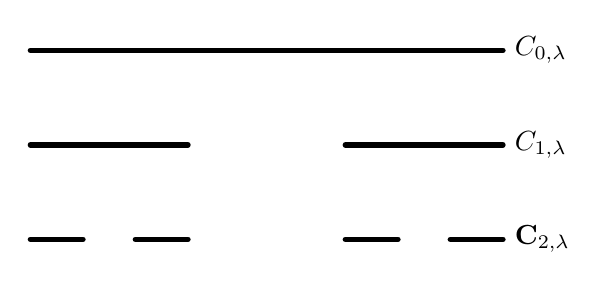
\begin{tikzpicture}[x=6cm, y=1.2cm, line cap=round, line width=2pt]
      \draw (0,0) -- (1,0) node[anchor=west]{\(C_{0, \lambda}\)};

      % \node[anchor=west] at (1.02,0) {\(\mathbf{C}_{0,\lambda}\)};

      \draw (0,-1) -- (1/3,-1);

      \draw (2/3,-1) -- (1,-1) node[anchor=west]{\(C_{1, \lambda}\)};

      % \node[anchor=west] at (1.02,-1) {\small \(\mathbf{C}_{1,\lambda}\)};

      \draw (0,-2) -- (1/9,-2);

      \draw (2/9,-2) -- (1/3,-2);

      \draw (2/3,-2) -- (7/9,-2);

      \draw (8/9,-2) -- (1,-2) node[anchor=west]{\(\mathbf{C}_{2,\lambda}\)};

      % \node[anchor=west] at (1.02,-2) {\(\mathbf{C}_{2,\lambda}\)};

      % \useasboundingbox (-0.05,-2.5) rectangle (1.1,0.5);
    \end{tikzpicture}
    \caption{Costruzione dell'insieme di Cantor \(C_\lambda\)}
  \end{figure}
  La funzione che vogliamo costruire sarà il limite della successione di
  funzioni monotone definite a partire dagli insiemi intermedi, indicati
  con \(\mathbf{C}_{n,\lambda}\):
  \[
    f_n(x)=\frac{1}{\abs{C_{n,\lambda}}} \int_{0}^{x} \chi_{C_{n,\lambda}}(u) \mathrm du
  \]
  Si può dimostrare\footnotemark
  % \footnote{Vedi "Analisi Reale, Giuseppe Molteni, APPENDICE A: CANTOR
  % E VOLTERRA"}
  come questa successione di funzioni chiaramente monotone sia di Cauchy
  in \(\mathcal{C}([0,1])\) con la norma dell'estremo superiore, convergendo
  quindi ad una funzione \(f\), anch'essa chiaramente monotona, e quindi
  sicuramente a variazione limitata.
  
  Questa funzione però non è assolutamente continua e si può vedere ad
  esempio con la caratterizzazione di queste funzioni data
  dall'Esercizio 4, infatti, per come è costruita \(f\) risulta una
  funzione a salti sui punti di \([0,1]\) che appartengono a
  \(C_\lambda\), con \(f\) suriettiva sul codominio \([0,1]\), abbiamo quindi:
  \(f(C_\lambda)=[0,1]\) ma \(\abs{C_\lambda}=0 \neq 1 = \abs{[0,1]}\)
\item Proviamo che l'inclusione \(\Lip([0,1])\subseteq AC([0,1])\) è stretta,
  ovvero che esiste almeno una funzione assolutamente continua che non è
  lipschitziana.
    
  Un esempio classico di funzione non lipschitziana è \(f(x)=\sqrt{x}\)
  infatti in \(x=0\) non è possibile trovare una costante di
  lipschitzianità valida poiché
  \[
    \forall K\in\mathbb{R^+}; \forall y\in[0,\frac{1}{K}]\cap [0,1],
    \abs{f(y)-f(0)}=\sqrt{y}\ge K\cdot y = K\cdot\abs{y-0}
  \]
  e quindi in tutto il sottointervallo \([0,\frac{1}{K}]\) la condizione
  per la lipschitzianità non è soddisfatta (il "problema" è
  evidentemente collegato al fatto che \(f'(x)\rightarrow +\infty\) per
  \(x\rightarrow 0^+\)).  Per dimostrare l'assoluta continuità utilizziamo il
  fatto noto\footnote{Proposizione 1.5.5,"Analisi Reale, Giuseppe
    Molteni, APPENDICE A: CANTOR E VOLTERRA"} per le funzioni integrali
  di funzioni Lebesgue-integrabili, infatti presa
  \[
    g(x)= \frac{2}{3}\cdot x^{\frac{3}{2}}
  \]
  chiaramente \(g\in L([0,1])\) e inoltre abbiamo che:
  \[
    f(x)=\int_0^x g(u) du
  \]
   
  \begin{center}
    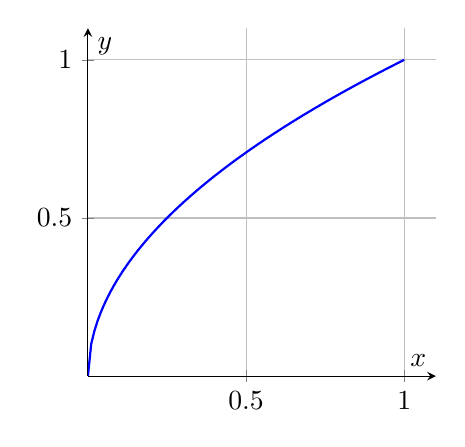
\begin{tikzpicture}
      \begin{axis}[ axis lines = middle, xlabel = \(x\), ylabel =
        {\(y\)}, domain=0:1, samples=100, width=6cm, height=6cm,
        grid=both, xmin=0, xmax=1.1, ymin=0, ymax=1.1, ]
        \addplot[blue, thick] {sqrt(x)};
      \end{axis}
    \end{tikzpicture}
  \end{center}

\item Proviamo che l'inclusione
  \(\mathcal{C}^1([0,1])\subseteq \Lip([0,1])\) è stretta, ovvero che esiste almeno una
  funzione Lipschitz che non è \(\mathcal{C^1}\).
    
  Una condizione semplice perché una funzione sia Lipschitz è che sia
  polinomiale, nel nostro esempio addirittura lineare, mentre per far
  cadere la condizione sulla continuità della derivata sia la presenza
  di un punto ``non-liscio'', viene quindi naturale la scelta di
  \[
    f(x)=\abs{x-\frac{1}{2}}
  \]
  \begin{itemize}
  \item \(f\) è Lipschitz, con costante di lipschitzianità \(K=1\)
    infatti:
    \(\forall x,y\in [0,\frac{1}{2}] \lor \forall x,y\in [\frac{1}{2},1]\) abbiamo che
    \[
      \abs{f(x)-f(y)} = \abs{\mp x\pm \frac{1}{2} \pm y \mp \frac{1}{2}}= 1\cdot
      \abs{x-y}
    \]
    se invece \(x\in[0,\frac{1}{2}] \land y\in [\frac{1}{2},1]\) (o
    viceversa) abbiamo che
    \[\abs{f(x)-f(y)}=
      \abs{-x+\frac{1}{2}-y+\frac{1}{2}}=\abs{x+y-1}\leq\abs{x-y}
    \]
    poiché \(x-1\leq -x\).
  \item \(f\) è chiaramente non \(\mathcal{C}^1\) perché la sua derivata è
    discontinua in 0.
  \end{itemize}
  \begin{center}
    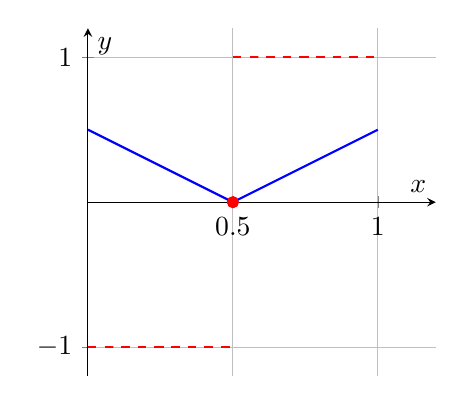
\begin{tikzpicture}
      \begin{axis}[ axis lines = middle, xlabel = \(x\), ylabel =
        {\(y\)}, domain=0:1, samples=100, width=6cm, height=6cm,
        grid=both, xmin=0, xmax=1.2, ymin=-1.2, ymax=1.2, ]
        % curva della funzione valore assoluto
        \addplot[blue, thick] {abs(x-0.5)};
        % derivata a sinistra
        \addplot[red, thick, dashed, domain=0:0.5] {-1};
        % derivata a destra
        \addplot[red, thick, dashed, domain=0.5:1] {1};
        % \node[red, anchor=south] at (0.9,1) {\(f'(x)\)};
    
        \addplot[red, only marks] coordinates {(0.5,0)};
        % \node[red, anchor=north] at (0.5,0) {\((\frac{1}{2},0)\)};
      \end{axis}
    \end{tikzpicture}
  \end{center}
\end{enumerate}

\footnotetext{Vedi "Analisi Reale, Giuseppe Molteni, APPENDICE A: CANTOR
  E VOLTERRA"}

%%% Local Variables:
%%% mode: LaTeX
%%% TeX-engine: luatex
%%% ispell-local-dictionary: "italian"
%%% TeX-master: "main"
%%% End:

